\section{Dashboard}
\label{sec:proposed:dashboard}

The dashboard is the visible surface of the proposed solution. Its
design is governed by three concerns. First, the dashboard must
serve five stakeholder groups whose analytical questions overlap
only partially. Second, every analyst must be able to bound the
analysis to the slice of the dataset that matters for their
question; the global filter set must be both expressive and
shared across views. Third, the visual design must follow
established storytelling principles~\cite{knaflic2015} so that the
analytical claims of Section~\ref{sec:proposed:modules} are
legible to non-technical stakeholders.

\subsection{Stakeholders and questions}

Five stakeholder groups are in scope. Each group asks a
different set of analytical questions; the dashboard maps each
group to a primary lens while leaving the remaining lenses
accessible. The mapping is summarised in
Table~\ref{tab:proposed:stakeholders}; the questions themselves
are taken from the advisor specification~\cite{thoai2025} and
elaborated for the HCMC operational context.

\begin{table}[H]
\centering
\caption{Stakeholders, primary questions, and primary lens.}
\label{tab:proposed:stakeholders}
\renewcommand{\arraystretch}{1.20}
\begin{tabularx}{\linewidth}{p{3.0cm}Xp{2.4cm}}
\hline
\textbf{Stakeholder} & \textbf{Primary questions} & \textbf{Primary lens} \\
\hline
MCPT operator / city planner
    & Which routes underperform the network? Which company is the worst on ghost rate? Where is ridership trending up or down? How is subsidy distributed?
    & Network, Financial \\

Bus company analyst
    & Are our trips actually completing? Do they keep to the planned headway? Where on the route do we lose time? Are our buses running near-empty?
    & Route, Financial \\

Student / worker commuter
    & When is my route at its busiest? How reliable is the schedule? Is there a less-crowded alternative?
    & Stop, Route \\

Business owner
    & When is foot-traffic high near my shop? Which routes feed the area? Is the morning commute reliable?
    & Stop \\

New bus user
    & Which route is beginner-friendly? How crowded does it get at peak? Where do I board?
    & Stop \\
\hline
\end{tabularx}
\end{table}

The dashboard is not partitioned by stakeholder: every lens is
available to every user. The mapping above identifies which lens
each user starts on; once inside, the MCV interaction model
(Section~\ref{sec:theory:mcv}) lets them drill into adjacent
lenses without losing filter context.

\subsection{Filter flexibility}

A second design concern is that the analytical questions in
Table~\ref{tab:proposed:stakeholders} all imply different slices
of the dataset. An MCPT operator asking ``which routes
underperform on weekday peak hours'' wants weekdays $\times$ 06--09
$+$ 17--20 hour bands; a student asking ``how busy is route 53 at
17:00 on Thursdays'' wants a stricter narrowing.
The dashboard exposes a single global filter bar that every lens
reads from. The filters are listed in
Table~\ref{tab:proposed:filters}; they compose multiplicatively
(any combination is valid) and they persist across lens switches.

\begin{table}[H]
\centering
\caption{Global filter set shared by all lenses.}
\label{tab:proposed:filters}
\begin{tabularx}{\linewidth}{p{3.0cm}p{4.4cm}X}
\hline
\textbf{Filter} & \textbf{Type} & \textbf{Default} \\
\hline
Date range          & calendar (start, end) & full available range \\
Day type            & multiselect: Weekday / Weekend / Holiday & all \\
Hour range          & dual slider 0--23     & 0--23 \\
Route               & multiselect on \texttt{route\_no} & all \\
Company             & multiselect on \texttt{company\_id} & all \\
Zone                & multiselect (HCMC ward) & all \\
\hline
\multicolumn{3}{l}{\emph{Selection state (lens-driven, not user-set)}} \\
Selected route      & set by Network treemap click or Route Explorer dropdown & none \\
Selected stop       & set by map click or Stop Analysis search & none \\
Active canvas       & set by canvas selector in the panel & \texttt{map} \\
\hline
\end{tabularx}
\end{table}

The filter bar is visually pinned at the top of the analysis
panel so it never falls below the fold. Every applied filter
appears as a coloured chip; default values are not shown so the
chip strip never clutters when the user has not narrowed the
analysis. This follows Knaflic's principle of removing visual
clutter that does not carry information~\cite{knaflic2015}.

\subsection{Layout}

The dashboard is a three-column shell on a single page,
illustrated in Figure~\ref{fig:proposed:layout}. A 52-pixel icon
strip on the far left switches between the five lenses (plus the
upcoming Ask-the-Data interface). A 360-pixel analysis panel in
the centre holds the filter bar, the lens header, the KPI grid,
the canvas selector, and the lens-specific drill-down lists. The
remainder of the viewport is the canvas itself, which renders one
of two things: the geospatial map (default) or a single
analytical chart selected from the panel.

\begin{figure}[H]
\centering
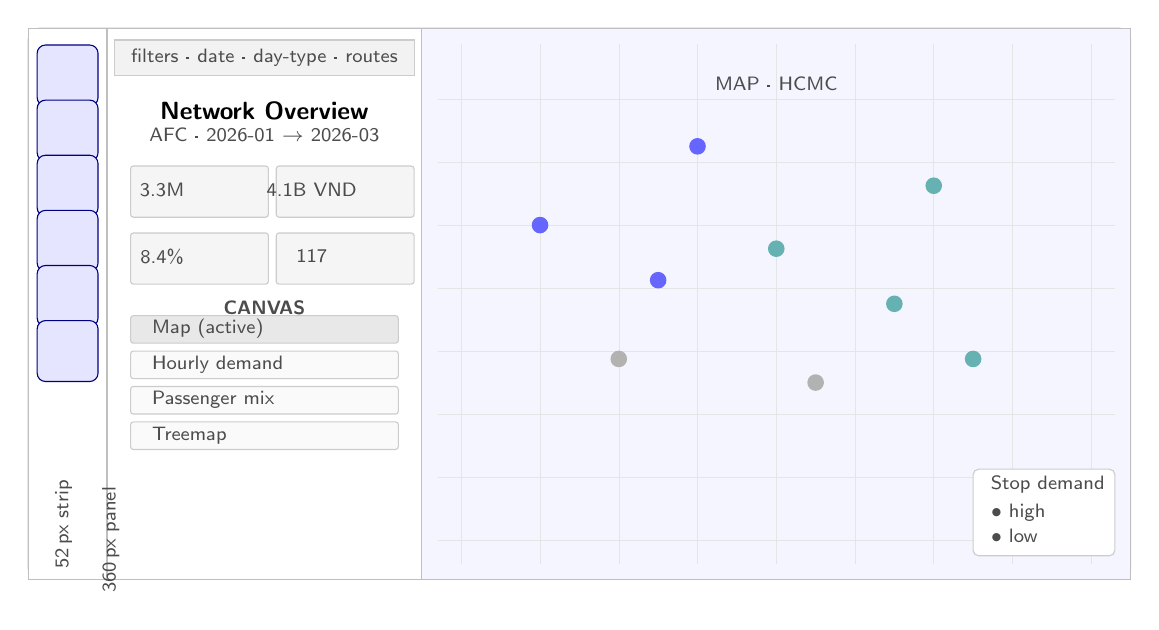
\begin{tikzpicture}[
    box/.style       ={rectangle, rounded corners=2pt,
                        font=\footnotesize\sffamily, align=center,
                        inner sep=4pt},
    icon/.style      ={rectangle, rounded corners=3pt,
                        draw=blue!50!black, fill=blue!10,
                        font=\small, minimum width=22pt,
                        minimum height=22pt, align=center},
    label/.style     ={font=\scriptsize\sffamily, color=gray!60!black},
]

\draw[draw=gray!50, rounded corners=4pt, fill=gray!2]
    (0,0) rectangle (14, 7);

% --- Icon strip ---
\draw[draw=gray!50, fill=white]
    (0,0) rectangle (1, 7);
\foreach \i in {0,1,2,3,4,5} {
    \node[icon] at (0.5, 6.4 - \i*0.7) {};
}
\node[label, rotate=90] at (0.45, 0.7) {52\,px strip};

% --- Analysis panel ---
\draw[draw=gray!50, fill=white]
    (1,0) rectangle (5, 7);

% Filter bar
\draw[draw=gray!40, fill=gray!10]
    (1.1, 6.4) rectangle (4.9, 6.85);
\node[label] at (3, 6.62) {filters · date · day-type · routes};

% Header
\node[box, font=\small\sffamily\bfseries] at (3, 5.95) {Network Overview};
\node[label] at (3, 5.65) {AFC · 2026-01 \(\rightarrow\) 2026-03};

% KPI grid
\foreach \r in {0,1} {
    \foreach \c in {0,1} {
        \draw[draw=gray!40, fill=gray!8, rounded corners=1pt]
            (1.3 + \c*1.85, 4.6 - \r*0.85) rectangle (3.05 + \c*1.85, 5.25 - \r*0.85);
    }
}
\node[label] at (1.7, 4.95) {3.3M};
\node[label] at (3.6, 4.95) {4.1B VND};
\node[label] at (1.7, 4.10) {8.4\%};
\node[label] at (3.6, 4.10) {117};

% Canvas selector
\node[label, font=\scriptsize\sffamily\bfseries] at (3, 3.45) {CANVAS};
\draw[draw=gray!40, fill=gray!18, rounded corners=1pt]
    (1.3, 3.0) rectangle (4.7, 3.35);
\node[label, anchor=west] at (1.45, 3.18) {Map (active)};
\foreach \i/\name in {1/Hourly demand, 2/Passenger mix, 3/Treemap} {
    \draw[draw=gray!40, fill=gray!4, rounded corners=1pt]
        (1.3, 3.0 - \i*0.45) rectangle (4.7, 3.35 - \i*0.45);
    \node[label, anchor=west] at (1.45, 3.18 - \i*0.45) {\name};
}

\node[label, rotate=90] at (1.05, 0.5) {360\,px panel};

% --- Canvas (map area) ---
\draw[draw=gray!50, fill=blue!4]
    (5,0) rectangle (14, 7);

\foreach \x in {5.5, 6.5, ..., 13.5}
    \draw[gray!20, very thin] (\x, 0.2) -- (\x, 6.8);
\foreach \y in {0.5, 1.3, ..., 6.5}
    \draw[gray!20, very thin] (5.2, \y) -- (13.8, \y);

\foreach \x/\y/\c in {6.5/4.5/blue, 8.0/3.8/blue, 9.5/4.2/teal,
                      11.0/3.5/teal, 7.5/2.8/gray, 10.0/2.5/gray,
                      12.0/2.8/teal, 8.5/5.5/blue, 11.5/5.0/teal} {
    \fill[\c!60] (\x, \y) circle (3pt);
}

\node[label] at (9.5, 6.3) {MAP · HCMC};

% Legend
\draw[draw=gray!40, fill=white, rounded corners=2pt]
    (12.0, 0.3) rectangle (13.8, 1.4);
\node[label, anchor=west] at (12.1, 1.20) {Stop demand};
\node[label, anchor=west] at (12.1, 0.85) {\(\bullet\)~high};
\node[label, anchor=west] at (12.1, 0.55) {\(\bullet\)~low};

\end{tikzpicture}
\caption{Three-column dashboard layout. The icon strip (52~px)
switches lenses; the analysis panel (360~px) holds filters, the
KPI grid and the canvas selector; the canvas (remainder of the
viewport) renders either the map or a single chart at a time.}
\label{fig:proposed:layout}
\end{figure}

Two binding rules govern the canvas: at most one chart is shown
at any time, and that chart fills at least 60\% of the viewport.
Liu's MCV literature~\cite{liu2022} shows that dense panels
crowded with small charts are a common failure mode of analytical
dashboards; Knaflic adds that an analyst's attention should be
directed to one analytical claim at a time~\cite{knaflic2015}.
The canvas-swap pattern enforces both: the panel renders no
charts of its own (only KPIs, lists, and selectors), and the
canvas renders one chart at canvas size --- typically 1500\,px
wide on a 1920\,px display.

\begin{figure}[H]
\centering
\includegraphics[width=0.95\linewidth]{images/screenshots/dashboard_network}
\caption{Dashboard with the Network Overview lens active and
the geospatial canvas in the default state. The icon strip is
on the far left; the analysis panel (filters, KPIs, canvas
selector, top-routes list) occupies the centre column; the
canvas occupies the remainder of the viewport.}
\label{fig:proposed:screenshot:network}
\end{figure}

\begin{figure}[H]
\centering
\includegraphics[width=0.95\linewidth]{images/screenshots/dashboard_route}
\caption{Dashboard with the Route Explorer lens active and
the QoS-2 distribution chart selected as the canvas. The map
returns one click away. Note that the panel itself contains
no charts --- only the lens-specific KPIs and the canvas
selector.}
\label{fig:proposed:screenshot:route}
\end{figure}

\subsection{Chart catalogue per lens}

Table~\ref{tab:proposed:charts} lists the chart that each canvas
option produces, alongside the analytical question it answers and
the literature primitive (where applicable) that grounds the
visualisation choice.

\begin{table}[H]
\centering
\caption{Chart catalogue. Each row is one canvas option in the
dashboard.}
\label{tab:proposed:charts}
\renewcommand{\arraystretch}{1.20}
\begin{tabularx}{\linewidth}{p{2.0cm}p{3.4cm}p{3.0cm}X}
\hline
\textbf{Lens} & \textbf{Canvas} & \textbf{Chart type} & \textbf{Question} \\
\hline
Network       & Hourly demand          & Stacked area, AM/PM bands & When does demand peak? \\
Network       & Passenger mix          & Donut, four segments      & Who rides? \\
Network       & Demand pattern cluster & Heatmap, GroupSet groups~\cite{liu2022} & Which routes share a daily shape? \\
Network       & Route health treemap   & Treemap, ghost-rate colour & Which routes underperform? \\
Network       & Operator scatter       & Bubble scatter            & How do companies compare? \\
\hline
Route         & Hourly demand          & Stacked area              & When is this route busy? \\
Route         & QoS-1 trend            & Daily line~\cite{srisakaokul2023} & Are scheduled trips actually running? \\
Route         & QoS-2 distribution     & Histogram~\cite{srisakaokul2023}  & How on-route are GPS trajectories? \\
Route         & QoS-3 box plot         & Per-stop box~\cite{srisakaokul2023} & Where on the route does delay accumulate? \\
Route         & Speed corridor         & Map polyline + FuzzyCut~\cite{liu2022} & Where is this route slow? \\
Route         & Trip Gantt             & Gantt, anomaly highlight  & How do trips line up across the day? \\
Route         & Tet vs.\ normal        & Side-by-side line         & How did Tet affect demand? \\
\hline
Stop          & Hourly demand          & Bar chart                 & When is this stop busy? \\
Stop          & Routes $\times$ hour   & Heatmap                   & Which routes feed this stop and when? \\
Stop          & Multi-stop comparison  & Radar, 2--4 stops         & How do these stops compare? \\
Stop          & Spatial accessibility  & Grid choropleth, Gridify~\cite{liu2022} & Which areas are underserved? \\
\hline
Financial     & Daily revenue          & Bar, weekday/weekend      & When does the network earn revenue? \\
Financial     & Payment channels       & Horizontal bar, \% labels & How do passengers pay? \\
Financial     & Worst ghost-rate routes& Ranked horizontal bar     & Which routes waste fuel? \\
Financial     & Revenue scatter        & Bubble scatter            & Who earns vs.\ who is subsidised? \\
Financial     & Revenue efficiency     & Histogram + FuzzyCut~\cite{liu2022} & How do we band routes by revenue? \\
\hline
Metro         & Feeder catchment       & Concentric rings on map   & How well do buses feed the metro? \\
\hline
\end{tabularx}
\end{table}

The chart-type column is deliberately conservative: stacked area
charts for time series, histograms for distributions, scatter
plots for two-variable relationships, treemap for hierarchical
size $+$ colour encoding. Knaflic argues that the analyst's
attention should be on the data and the analytical claim, not on
the novelty of the chart~\cite{knaflic2015}; the dashboard
therefore prefers the canonical chart type for each question over
a more ornate alternative.

\subsection{Cross-lens interactions}

The MCV interaction model (Section~\ref{sec:theory:mcv}) connects
the lenses into a coherent dashboard. Three cross-lens
interactions are particularly relevant in practice.

\paragraph{Treemap tile $\rightarrow$ Route Explorer.}
A click on any tile in the Network route-health treemap sets the
\texttt{selected\_route} field in the shared session-state object
and switches the active lens to Route Explorer. The filter bar is
preserved, so the analyst arrives at the route-level view already
narrowed to the date range, day type, and hour band that were
active in the treemap.

\paragraph{Map stop $\rightarrow$ Stop Analysis.}
A click on any stop on the geospatial canvas sets
\texttt{selected\_stop\_key} and switches to Stop Analysis. The
panel re-populates with the boardings, dwell, and per-route
breakdown for the chosen stop, again preserving the global
filter context.

\begin{figure}[H]
\centering
\includegraphics[width=0.95\linewidth]{images/screenshots/dashboard_stop}
\caption{Stop Analysis lens reached by clicking a stop on the
geospatial canvas. The selected stop's boardings, peak hour,
average fare, and routes-served list populate the panel without
any explicit filter change by the analyst.}
\label{fig:proposed:screenshot:stop}
\end{figure}

\paragraph{Worst-ghost ranking $\rightarrow$ Route Explorer
$+$ ghost-only filter.} A click on a route in the Financial
worst-ghost ranking switches to Route Explorer with the route
selected and an additional filter applied that scopes the canvas
to only the trips classified as near-ghost. This is the
``drill-from-symptom-to-cause'' pattern advocated by
Knaflic~\cite{knaflic2015}: the analyst sees an anomaly in
aggregate, clicks once, and lands at the trip-level view that
explains it.
